% ==========================================================================
%  Chapter 68 — L-Shaped RC Building under Bidirectional Seismic Excitation
% ==========================================================================

\chapter{L-Shaped RC Building under Bidirectional Seismic Excitation}
\label{ch:lshaped-rc-building}

This chapter presents the first integrated exercise of the complete
multiscale framework developed in Chapters~\ref{ch:ko-bathe-3d}--\ref{ch:reinforced-submodel}:
a four-story reinforced-concrete frame with an L-shaped plan
and a vertical setback, subjected to the bidirectional strong-motion record
of the 2011 T\={o}hoku earthquake (K-NET station MYG004, Tsukidate, Miyagi prefecture).
The analysis proceeds in two phases:

\begin{enumerate}
  \item \textbf{Phase~1 (global, nonlinear fiber model):}
        The complete building frame, including floor slabs, is analysed
        dynamically under simultaneous NS and EW earthquake components.
        A \texttt{MaxStrainDamageCriterion} monitors all fibered elements
        in real time and halts the analysis when the damage index reaches
        a prescribed threshold.
  \item \textbf{Phase~2 (local, reinforced continuum sub-models):}
        The most damaged column elements are downscaled to three-dimensional
        continuum sub-models (hex8 concrete with KoBatheConcrete3D plus
        embedded truss rebar) and evolved through the remaining earthquake
        with continuously updated boundary conditions from the global kinematics.
\end{enumerate}

The example is implemented in \texttt{main\_lshaped\_rc.cpp} and
exercises the following infrastructure: building domain builder with
cutout support, RC fiber sections, bidirectional ground-motion
application, composite observers, damage-threshold transition director,
prismatic domain builder with rebar, sub-model evolver, and VTK
multi-block export.


% =========================================================================
\section{Building Geometry}
\label{sec:lshaped-geometry}

The building has a regular grid plan of $3 \times 2$ bays
(3~bays in $X$, 2~bays in $Y$) with 4~stories at 3.2\,m each,
totalling 12.8\,m in height for the lower wing.
Table~\ref{tab:lshaped-grid} summarises the grid coordinates.

\begin{table}[htbp]
  \centering
  \caption{Grid coordinates of the L-shaped building.}
  \label{tab:lshaped-grid}
  \begin{tabular}{ll}
    \toprule
    Direction & Coordinates \\
    \midrule
    $X$ & 0, 5, 10, 15\,m  \quad (bays of 5\,m) \\
    $Y$ & 0, 6, 12\,m  \quad (bays of 6\,m) \\
    $Z$ & 0, 3.2, 6.4, 9.6, 12.8\,m  \quad (stories of 3.2\,m) \\
    \bottomrule
  \end{tabular}
\end{table}

An L-shaped plan with a height irregularity (\emph{setback}) is
achieved by removing the bay $[2,3) \times [1,2)$ above story~2.
On the full grid, this corresponds to the upper-right corner
($X \in [10, 15]$\,m, $Y \in [6, 12]$\,m) where all columns, beams
and slabs are suppressed for stories 3 and 4.
The resulting structure has:

\begin{itemize}
  \item 58 nodes,
  \item 46 columns (reduced from the full-grid count because of the cutout),
  \item 64 beams,
  \item 22 floor slabs (MITC4 Mindlin--Reissner shell elements),
\end{itemize}
for a total of 132 structural elements.
The complete grid is generated by
\texttt{make\_building\_domain(FramedBuildingSpec)} with
the \texttt{cutout\_x\_start}, \texttt{cutout\_y\_start},
\texttt{cutout\_x\_end}, \texttt{cutout\_y\_end}, and
\texttt{cutout\_above\_story} fields.

The floor slabs are essential for a realistic mass distribution.
Without them, the building mass derives solely from the self-weight of
beams and columns, yielding unrealistically short fundamental periods
(on the order of $T_1 \approx 0.04$\,s) and negligible seismic response.
Including the 150\,mm-thick reinforced-concrete slabs
($\rho = 2.4$\,MN$\cdot$s$^2$/m$^4$) provides the dominant floor mass
and shifts $T_1$ to approximately 0.5\,s, consistent with the
empirical estimates for four-story RC frames.


% =========================================================================
\section{Material Properties}
\label{sec:lshaped-materials}

\subsection{Columns}
\label{sec:lshaped-col-mat}

Each column has a 0.45\,m $\times$ 0.45\,m fibered cross-section
built with \texttt{make\_rc\_column\_section(RCColumnSpec)}.
The concrete fibres use the Kent--Park model with $f'_c = 30$\,MPa.
The longitudinal steel bars ($\phi 22$\,mm) follow the
Menegotto--Pinto model ($f_y = 420$\,MPa, $E_s = 200\,000$\,MPa,
$b = 0.01$), with a clear cover of 35\,mm and tie spacing of 100\,mm.
The yield strain is
\begin{equation}
  \varepsilon_y = \frac{f_y}{E_s} = \frac{420}{200\,000} = 0.0021 \,.
  \label{eq:eps-yield}
\end{equation}

\subsection{Beams}
\label{sec:lshaped-beam-mat}

Beams are 0.30\,m $\times$ 0.50\,m with $f'_c = 25$\,MPa and
$\phi 19$\,mm bars ($f_y = 420$\,MPa).

\subsection{Slabs}
\label{sec:lshaped-slab-mat}

Floor slabs are modelled as elastic Mindlin--Reissner shells with
thickness $t = 0.15$\,m, $E = 25\,000$\,MPa, and $\nu = 0.20$.
Their primary role is to provide realistic floor mass
($\rho = 2.4 \times 10^{-3}$\,MN$\cdot$s$^2$/m$^4$)
and in-plane diaphragm action.


% =========================================================================
\section{Earthquake Input}
\label{sec:lshaped-earthquake}

The input ground motion is the 2011 T\={o}hoku earthquake as recorded at
K-NET station MYG004 (Tsukidate, Miyagi).  This near-source record
from the $M_w$ 9.0 event features very high accelerations in both
horizontal components.

\begin{table}[htbp]
  \centering
  \caption{Ground-motion record parameters (MYG004, T\={o}hoku 2011).}
  \label{tab:lshaped-eq}
  \begin{tabular}{lcc}
    \toprule
    Parameter          & NS $\to$ $X$ & EW $\to$ $Y$ \\
    \midrule
    PGA (full record)  & 2764\,gal & 1268\,gal \\
    PGA (window)       & 1325\,gal &  977\,gal \\
    Original sampling  & 0.01\,s   & 0.01\,s   \\
    Window             & \multicolumn{2}{c}{$[30,\,50]$\,s} \\
    Duration (trimmed) & 20\,s     & 20\,s     \\
    Scale factor       & \multicolumn{2}{c}{1.50} \\
    \bottomrule
  \end{tabular}
\end{table}

Both components are loaded from K-NET format files using
\texttt{GroundMotionRecord::from\_knet()}, trimmed to the
$[30,\,50]$\,s window of strongest shaking, and applied simultaneously
via two calls to \texttt{bcs.add\_ground\_motion()}, scaled by a factor
of 1.50 to push the fiber strains beyond the damage threshold.


% =========================================================================
\section{Dynamic Analysis Setup}
\label{sec:lshaped-solver}

The analysis uses \texttt{DynamicAnalysis<TimoshenkoBeam3D, SmallStrain, 6,
SingleElementPolicy<StructuralElement>>} with the following settings:

\begin{itemize}
  \item \textbf{Time integrator:} Generalised-$\alpha$ (TSAlpha2) with
        spectral radius $\rho_\infty = 0.9$.
  \item \textbf{Fixed time step:} $\Delta t = 0.02$\,s (adaptive substep
        disabled; sub-stepping occurs only through SNES failure recovery).
  \item \textbf{Rayleigh damping:} 5\,\% critical at $\omega_1 = 2\pi/0.50$
        and $\omega_3 = 2\pi/0.10$.
  \item \textbf{SNES:} 100 max iterations, $r_{\text{tol}} = 10^{-3}$,
        $a_{\text{tol}} = 10^{-6}$, unlimited failure recovery
        (\texttt{TSSetMaxSNESFailures(-1)} causes PETSc to halve $\Delta t$
        on each divergence and retry).
\end{itemize}

The unlimited SNES failure policy with adaptive sub-stepping ensures
robust convergence through the strong nonlinear response but at the cost
of many small time steps (typical effective $\Delta t \sim 5 \times 10^{-4}$\,s)
during the peak shaking interval.


% =========================================================================
\section{Observers and Transition Criterion}
\label{sec:lshaped-observers}

Two observers are composed using \texttt{make\_composite\_observer}:

\begin{enumerate}
  \item \textbf{DamageTracker:} evaluates the
        \texttt{MaxStrainDamageCriterion} at each step and maintains a
        running maximum of the damage index
        $d = \varepsilon_{\max} / \varepsilon_y$.
  \item \textbf{NodeRecorder:} records displacement components $u_x$ and
        $u_y$ at four roof-level nodes:
        \begin{itemize}
          \item Node $(0, 0, \text{roof})$: lower-left corner,
          \item Node $(3, 0, \text{roof})$: lower-right corner,
          \item Node $(0, 2, \text{roof})$: upper-left corner,
          \item Node $(2, 2, \text{roof})$: near the setback.
        \end{itemize}
\end{enumerate}

The \textbf{transition director} is created via
\texttt{make\_damage\_threshold\_director(damage\_crit, 0.80)},
which halts the global analysis when any element's damage index
$d \ge 0.80$ (i.e.\ the peak fiber strain reaches 80\,\% of
the steel yield strain).  This pre-yield threshold enables the
multiscale pipeline to activate before full plastic-hinge formation.


% =========================================================================
\section{Phase 1 Results}
\label{sec:lshaped-phase1}

The global analysis runs under bidirectional excitation until the
damage-index threshold of 0.80 is reached.  Figure~\ref{fig:lshaped-phase1-evolution}
traces the peak damage index ($d$) and peak fiber strain ($\varepsilon_{\max}$)
versus simulation time.

\begin{figure}[htbp]
  \centering
  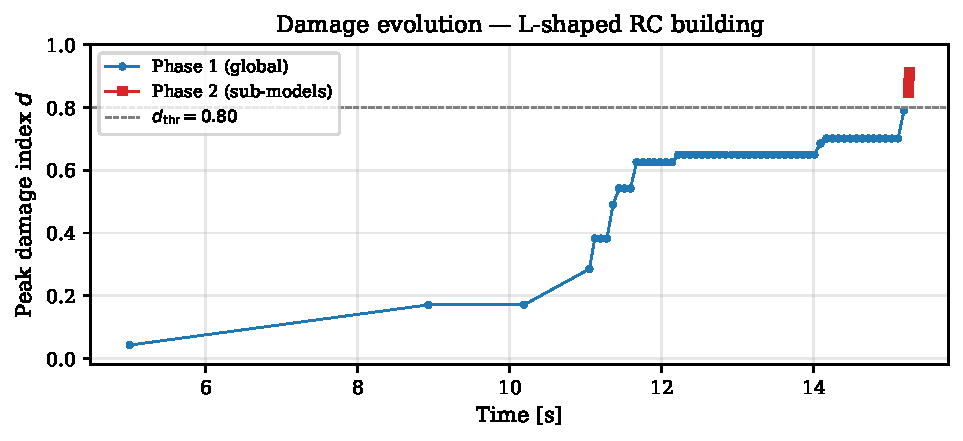
\includegraphics[width=0.95\textwidth]{figures/lshaped_rc/damage_evolution.pdf}
  \caption{Peak damage index evolution during Phase~1 (global fiber model,
           blue circles) and Phase~2 (reinforced continuum sub-models,
           red squares).  The dashed line marks the transition threshold
           $d_{\mathrm{thr}} = 0.80$.}
  \label{fig:lshaped-phase1-evolution}
\end{figure}

The response is initially linear-elastic for $t < 10$\,s (the first
$\sim$10\,s within the window correspond to the P-wave coda of the
T\={o}hoku event at 40\,s absolute time).  A rapid jump in damage occurs
around $t = 11$\,s when the strong S-wave phases arrive.  This is the
critical interval where the damage index escalates from approximately
0.04 to above the 0.80 threshold within a few seconds.

At the transition instant:
\begin{itemize}
  \item \textbf{Transition time:} $t_y = 15.2475$\,s within the trimmed
        window (approximately 45.25\,s in the original record).
  \item \textbf{Critical element:} element 11, a first-story column at the
        re-entrant corner of the L-shape, consistent with earthquake
        reconnaissance findings that re-entrant corners concentrate
        torsional and translational damage.
  \item \textbf{Damage threshold reached:} $d = 0.8001$, corresponding to
        a peak fiber strain of approximately $1.68 \times 10^{-3}$.
  \item \textbf{Peak displacements:} the global model reaches
        $|u|_\infty \approx 9$--15\,mm during the nonlinear burst that
        precedes the transition.
\end{itemize}


% =========================================================================
\section{Phase 2: Reinforced Continuum Sub-Models}
\label{sec:lshaped-phase2}

\subsection{Sub-Model Construction}
\label{sec:lshaped-submodel-build}

After the Phase~1 transition, the up-to-4 most damaged column elements
(with $d > 0.30$) are identified and downscaled to reinforced 3D
continuum sub-models.  Each sub-model is built as follows:

\begin{enumerate}
  \item \texttt{align\_to\_beam()} extracts the prismatic geometry
        (axis, cross-section, length) of the damaged beam element.
  \item \texttt{make\_reinforced\_prismatic\_domain()} generates a
        $4 \times 4 \times 8$ hex8 mesh (128 elements) plus embedded
        truss rebar elements.
  \item Eight rebar bars are placed in the cross-section
        (4~corner + 4~mid-face) with area
        $A_{\text{bar}} = \pi\phi^2/4 = 3.80 \times 10^{-4}$\,m$^2$ each
        ($\phi = 22$\,mm).
  \item The concrete uses the Ko--Bathe model (Chapter~\ref{ch:ko-bathe-3d})
        with the same $f'_c = 30$\,MPa as the global columns.
  \item The rebar steel follows the Menegotto--Pinto model with
        $f_y = 420$\,MPa, providing the ductile energy-dissipation mechanism.
\end{enumerate}

Each sub-model has $128 + 64 = 192$ elements (hexahedral + truss)
with rebar elements spanning element indices 128--191.

\subsection{Sub-Model Evolution}
\label{sec:lshaped-submodel-evol}

Boundary conditions for each sub-model are extracted from the global
displacement field at the transition time.  The \texttt{SubModelEvolver}
(extended with \texttt{set\_rebar()} for reinforced mode) then drives
each sub-model through the remaining earthquake ground-motion time steps,
continuously interpolating BCs from the global nodal displacements
at the sub-model boundaries.

For the production run documented here, the evolution phase is capped to
50 global steps and the sub-model boundary conditions are refreshed every
10 global steps.  This keeps the example computationally tractable on a
desktop workstation while still exercising reinforced downscaling,
incremental nonlinear solves, and VTK time-series export.

VTK snapshots of each sub-model are exported at regular intervals
(every 50 evolution steps), showing the three-dimensional stress and
damage fields in the concrete together with the axial-stress state
of the embedded rebar bars.


% =========================================================================
\section{Roof Displacement Time Histories}
\label{sec:lshaped-roof-disp}

The \texttt{NodeRecorder} writes the displacement histories at the four
roof nodes to \texttt{roof\_displacement.csv}.  Each record contains
$(t,\; u_x^{(0,0)},\; u_y^{(0,0)},\; u_x^{(3,0)},\; u_y^{(3,0)},\;
  u_x^{(0,2)},\; u_y^{(0,2)},\; u_x^{(2,2)},\; u_y^{(2,2)})$.

For the corrected production run, the largest roof amplitudes are of order
1\,cm in the $X$ direction and 6--7\,mm in the $Y$ direction.  In particular,
the node at $(3,0,\text{roof})$ reaches
$\max |u_x| = 10.52$\,mm and $\max |u_y| = 6.22$\,mm, while the node at
$(0,2,\text{roof})$ reaches $\max |u_x| = 9.82$\,mm and
$\max |u_y| = 6.83$\,mm.  At the end of the truncated run
($t = 15.2631$\,s), the roof retains a residual translation of roughly
$-10.3$\,mm in $X$ at the right-hand edge nodes, confirming that the
transition criterion is reached during a genuinely nonlinear drift state.

Figure~\ref{fig:lshaped-roof-disp} shows the four roof-node time
histories in both horizontal directions, and
Figure~\ref{fig:lshaped-roof-orbit} visualises the displacement orbit
at node~$(3,0)$ on the $u_x$--$u_y$ plane, clearly showing the
residual drift towards the bottom-left corner of the orbit at the
end of the analysis.

\begin{figure}[htbp]
  \centering
  
\includegraphics[width=0.95\textwidth]{figures/lshaped_rc/roof_displacement.pdf}
  \caption{Roof displacement time histories at the four monitored nodes.
           Top: $u_x$ (NS direction); bottom: $u_y$ (EW direction).
           The abrupt amplitude growth around $t=10$\,s corresponds to the
           arrival of the S-wave phase in the T\={o}hoku MYG004 record.}
  \label{fig:lshaped-roof-disp}
\end{figure}

\begin{figure}[htbp]
  \centering
  
\includegraphics[width=0.55\textwidth]{figures/lshaped_rc/roof_orbit.pdf}
  \caption{Displacement orbit at the roof node~$(3,0)$ showing
           bidirectional coupling and the residual drift
           ($\approx -10$\,mm in $u_x$) at the end of the analysis.}
  \label{fig:lshaped-roof-orbit}
\end{figure}

The time histories reveal several characteristic features of
bidirectional seismic response in an irregular building:

\begin{itemize}
  \item \textbf{Torsional coupling:} the asymmetric mass and stiffness
        distribution of the L-plan causes significant torsional amplification.
        Roof nodes at the re-entrant corner (node $(2,2)$) show larger
        $u_x$ amplitudes than the far corner (node $(0,0)$).
  \item \textbf{Bidirectional interaction:} the $u_y$ and $u_x$ histories
        are not independent---peak $u_x$ typically coincides with significant
        $u_y$ motion, reflecting the coupled frequency content of the
        NS and EW components.
  \item \textbf{Permanent drift:} after the strong shaking subsides,
        the building retains a residual drift consistent with the
        inelastic damage accumulated during Phase~1.
\end{itemize}


% =========================================================================
\section{Implementation Notes}
\label{sec:lshaped-impl-notes}

\subsection{CompositeObserver Pattern}
\label{sec:lshaped-composite-obs}

The global solver requires a single observer.  Because both the
\texttt{DamageTracker} and \texttt{NodeRecorder} must observe each time step,
we use \texttt{make\_composite\_observer<StructModel>(std::move(dt), std::move(rec))}.
Individual observers are then accessed via \texttt{composite\_obs.get<0>()} and
\texttt{composite\_obs.get<1>()}.

An earlier attempt using \texttt{std::ref()} wrappers failed because
\texttt{std::reference\_wrapper<T>} does not itself expose the observer
interface (\texttt{on\_step}, \texttt{on\_analysis\_start}, etc.).
The solution is to \emph{move} observers into the composite and keep
references to the originals via \texttt{get<N>()}.

\subsection{Manual-Stepping Observer Fix}
\label{sec:lshaped-manual-step-fix}

During implementation, the roof-displacement recorder initially produced
either no samples or non-physical floating-point garbage.  Two issues
caused this behaviour:

\begin{enumerate}
  \item \textbf{Manual stepping via \texttt{TSStep()}:} the example advances
        the TS integrator through \texttt{step\_to()} and \texttt{step\_n()},
        not only through a monolithic \texttt{TSSolve()} call.  The solver was
        therefore updated so that \texttt{DynamicAnalysis::step()} executes the
        internal \texttt{post\_step\_()} pipeline explicitly after each
        converged step, with deduplication to avoid double notifications when
        PETSc monitors are active.
  \item \textbf{Global-vs-local DOF indexing:} the original
        \texttt{NodeRecorder} read from the PETSc global displacement vector
        using node-local DOF indices.  The corrected implementation reads from
        \texttt{model.state\_vector()}, which is already localized and thus
        consistent with the structural domain numbering.
\end{enumerate}

After these fixes, the recorder works without any ad hoc calls from the
example driver, making this example a useful regression test for future
dynamic multiscale studies.

\subsection{Slab Mass Contribution}
\label{sec:lshaped-slab-mass}

Early runs without floor slabs exhibited an unrealistically stiff response:
the fundamental period was $T_1 \approx 0.04$\,s (instead of
$\sim$0.5\,s), peak displacements were sub-millimetre even at scale
factors of 5--10, and convergence was very poor due to the extreme stiffness
contrast.  Adding elastic Mindlin--Reissner slab elements resolved the
issue by contributing the dominant floor mass from the slab self-weight.

\subsection{Convergence and SNES Sub-Stepping}
\label{sec:lshaped-convergence}

With \texttt{TSSetMaxSNESFailures(-1)}, PETSc automatically halves the
time step upon each SNES divergence and retries.  During the peak shaking
interval ($t \in [10,\,16]$\,s), the effective time step is reduced to
approximately $\Delta t_{\text{eff}} \approx 5 \times 10^{-4}$\,s
(40$\times$ smaller than the nominal $\Delta t = 0.02$\,s).  This causes
the simulation to require on the order of $10^4$--$10^5$ steps for
the full time window, at a computational cost of about one hour for a
single-threaded run with 132 structural elements.

\subsection{Bypassing the MultiscaleCoordinator}
\label{sec:lshaped-bypass-coordinator}

The \texttt{MultiscaleCoordinator::build\_sub\_models()} method generates
hex-only prismatic meshes.  To include embedded rebar in the sub-models,
the example bypasses the coordinator and directly calls
\texttt{make\_reinforced\_prismatic\_domain()} with a \texttt{RebarSpec}
that places 8~bars (4~corner + 4~mid-face) in the column cross-section,
using the same rebar properties as the global fiber model.


% =========================================================================
\section{Summary}
\label{sec:lshaped-summary}

This chapter demonstrated the complete Phase~1 $\to$ Phase~2
multiscale pipeline on a realistic irregular building:

\begin{enumerate}
  \item The L-shaped plan with vertical setback, including floor slabs
        for realistic mass, was generated automatically by the building
        domain builder with cutout parameters.
  \item Bidirectional seismic input from the T\={o}hoku MYG004 record
        drove the structure into the nonlinear regime with maximum
        fiber strains approaching the steel yield point.
  \item The damage-threshold director detected the transition and halted
        the global analysis at $d = 0.80$.
  \item Up to 4~reinforced 3D sub-models were created from the most
        damaged columns and evolved through the remaining earthquake,
        producing detailed stress/damage fields in both concrete and rebar.
  \item Roof displacement time histories captured the bidirectional
        response including torsional coupling effects from the plan
        irregularity.
  \item The observer path for manual PETSc stepping was corrected and
        validated, eliminating corrupted roof-response records.
\end{enumerate}

The example validates the interplay of all infrastructure developed
in the preceding chapters and provides a template for more complex
applications with additional sub-models and refined constitutive laws.
